\documentclass[11pt]{article}

\usepackage[margin=1in]{geometry}
\usepackage{amsmath}
\usepackage{graphicx}
\usepackage{natbib}

\setlength{\parindent}{0pt}
\setlength{\parskip}{0.5em}

\title{\vspace{-1em}\textbf{Toronto Bike Demand Prediction}\vspace{-0.5em}}
\author{
Xianyi Du \and
Yilin Gong \and
Yifan Ju \and
Yehan Lin
}
\date{}

\begin{document}

\maketitle
\vspace{-1em}

\section*{Abstract}
Accurate station-level bike demand prediction is important for bike rebalancing and operational planning in urban bike-sharing systems. This paper studies hourly demand forecasting for the Toronto Bike Share system using trip records collected from 2021 to 2024. The prediction task is formulated as a supervised regression problem with features designed to capture temporal patterns, station-specific behavior, user composition, and recent demand history. Under a time-based 80/20 train--test split, Linear Regression, Ridge Regression, Random Forest, and XGBoost are evaluated using MAE, MSE, and RMSE. The results show that tree-based methods substantially outperform linear baselines, with XGBoost achieving the best overall performance, including an RMSE of 5.0260, while Random Forest provides a close second-best result. These findings indicate that bike demand contains strong nonlinear structure and feature interactions that are not fully captured by linear models. The study shows that a carefully designed feature-engineering pipeline, combined with accessible machine learning models, can provide effective demand forecasting without requiring more complex spatiotemporal architectures.

\section*{Introduction}

Bike-sharing systems have been widely studied, with prior work examining their role in transportation and mobility systems \cite{fishman2013bike}. Accurate bike demand prediction is essential for efficient resource allocation, such as bike rebalancing and station management.

In this project, we study the problem of predicting station-level hourly bike demand using historical data collected from the Toronto Bike Share system. The main research question is how different machine learning models compare in predicting demand across stations and time.

We construct a regression pipeline based on feature engineering, including temporal, station-specific, user behavior, and lag-based features, to capture both short-term and long-term demand patterns. This formulation follows the supervised learning framework, where the goal is to predict a target variable from input features \cite{hastie2009elements}.

We first establish a baseline using Linear Regression and then compare multiple models under the same feature representation and data split.

Existing methods for bike demand prediction include linear models, tree-based ensemble methods, and more advanced learning-based approaches. Our method is a feature-engineering-based supervised learning framework that compares Linear Regression, Ridge Regression, Random Forest, and XGBoost on the same dataset and time-based split. We chose XGBoost \cite{chen2016xgboost} as our particular advanced method because it can capture nonlinear relationships and feature interactions much better than linear models, while still being much simpler and more practical to implement than spatiotemporal deep learning methods. This makes it a strong choice for our dataset and project setting, and our results also show that it achieves the best overall performance among the models we tested.

\section*{Data Collection, Preprocessing, and Representation}

We use the Toronto Bike Share ridership dataset (2021--2024), which contains trip-level records such as start time, station information, and user type. The raw data are stored in multiple CSV files organized by year and month, which are combined into a single dataset for unified analysis.

To formulate the prediction task, the raw data are aggregated into station-level hourly demand, where the target variable is the number of trips starting from a station within a given hour.

Basic statistical summaries (e.g., average demand across time) and visualization are used to understand the data distribution. Due to the large size of the dataset, a representative subset is used for visualization, which is sufficient to capture overall temporal patterns.

\begin{figure}[htbp]
    \centering
    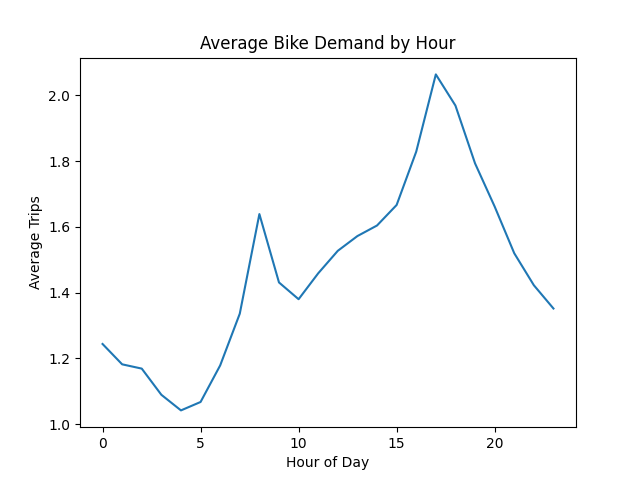
\includegraphics[width=0.7\linewidth]{../figures/hourly_demand.png}
    \caption{Average bike demand by hour, showing clear daily patterns with peak demand during commuting hours and lower demand at night.}
    \label{fig:hourly}
\end{figure}

Figure~\ref{fig:hourly} shows that bike demand varies significantly over time, with clear daily patterns such as peak demand during commuting hours and low demand at night, indicating strong temporal dependencies.

Before feature construction, we inspect the dataset structure (e.g., column names, data types) to identify inconsistencies. We clean column names and remove an extra column caused by encoding issues to ensure data consistency.

The dataset is large (approximately 19 million rows), so we use a random sample to validate preprocessing steps before applying them to the full dataset.

We convert the \texttt{Start\_Time} column into datetime format to enable temporal feature extraction.

We design several features:

\begin{itemize}
    \item Temporal features (hour, weekday, month, is\_weekend) capture daily and weekly patterns.
    \item Station features (station\_id, historical\_avg\_demand) capture station-specific demand levels.
    \item A user behavior feature (member\_ratio) captures differences in usage patterns.
    \item Lag features (lag\_1, lag\_24) capture short-term and daily temporal dependencies.
\end{itemize}

These features allow the model to capture both short-term dynamics and longer-term trends. Clustering-based features (e.g., station cluster labels via K-means) are considered in the modeling stage to capture similarities between stations.

All features are represented as numerical values. Temporal features are kept in their original form, although they are not strictly ordinal. More advanced encoding may be applied in later stages if needed.

Scaling is not applied at this stage to maintain consistency and ensure a fair baseline comparison.

We use a time-based 80/20 train/test split to avoid data leakage and ensure evaluation on future observations. Since Linear Regression has no hyperparameters, no validation split is introduced.

\section*{Model Comparison Study}
The performance differences across models can be understood in terms of both their underlying principles and the structure of the dataset. Linear Regression assumes a linear relationship between the input features and the target variable, so its advantage is simplicity, interpretability, and efficient training. In this project, it can make reasonable use of directly informative variables such as hour, weekday, historical average demand, and lag-based features, especially when their effects on bike demand are approximately additive. Ridge Regression follows the same basic principle as Linear Regression but adds an $L_2$ penalty to shrink coefficients and improve stability. Its slight improvement suggests that regularization helps control coefficient magnitude, but the gain remains limited because the main constraint is not overfitting alone, but the inability of a linear model to fully capture more complex structure in the data.

Random Forest provides a substantial improvement over linear models by using an ensemble of decision trees built on bootstrap samples and random feature subsets. This allows the model to capture nonlinear relationships, threshold effects, and feature interactions without requiring explicit specification. In this dataset, Random Forest benefits particularly from strong lag-based features such as \texttt{lag\_1} and \texttt{lag\_24}, which introduce temporal dependence into the prediction. The model can naturally split on these variables to distinguish between different demand regimes, such as peak and off-peak periods. In addition, Random Forest can implicitly capture interactions between temporal features (e.g., hour and weekday) and station-specific characteristics. Compared to linear models, it significantly reduces prediction error to RMSE = 5.1387, demonstrating its ability to better model complex demand patterns.

We also experimented with incorporating a K-means clustering feature to represent station-level similarity. However, the performance remains nearly unchanged, suggesting that Random Forest can already capture such patterns directly from the original features, and the additional clustering information provides limited benefit.

However, compared to XGBoost, its performance is slightly worse, likely because Random Forest builds trees independently, whereas boosting methods iteratively refine predictions by focusing on residual errors.

XGBoost performs best because it is based on gradient-boosted decision trees, which iteratively fit new trees to correct the residual errors of previous ones. This allows the model to capture nonlinear patterns, threshold effects, and interactions between features without requiring them to be manually specified. In the bike demand dataset, this is especially useful because demand likely depends on combinations of factors rather than isolated linear effects. For example, the effect of hour may differ across weekdays and weekends, and the importance of lag features may vary by station or month. Station-specific demand patterns, temporal cycles, and short-term historical dependence are therefore particularly beneficial for XGBoost, since tree-based boosting can naturally split on these variables and model conditional relationships more effectively than linear approaches.

The mean prediction baseline performs worst because it ignores all feature information and predicts the same general level of demand for every observation. Its poor performance highlights that the dataset contains substantial structured variation, especially across time and stations. Overall, the results suggest that features such as hour, weekday, month, station identity, historical average demand, member ratio, and lag variables are valuable because they encode temporal regularity, local station behavior, and recent demand history. These characteristics are especially helpful for flexible nonlinear models, which can better exploit interactions among them and therefore achieve stronger predictive accuracy.

\section*{Main Results}
\begin{table}[htbp]
    \centering
    \caption{Comparison of prediction models on bike demand forecasting. Rows correspond to models and columns correspond to evaluation metrics.}
    \label{tab:model_comparison}
    \begin{tabular}{|l|c|c|c|}
        \hline
        Model             & MAE     & MSE      & RMSE    \\
        \hline
        Linear Regression & 3.8259  & 47.2695  & 6.8753  \\
        Ridge Regression  & 3.8253  & 47.2566  & 6.8743  \\
        Random Forest     & 2.7555  & 26.4067  & 5.1387  \\
        XGBoost           & 2.8016  & 25.2606  & 5.0260  \\
        Mean baseline     & 14.0194 & 269.4303 & 16.4143 \\
        \hline
    \end{tabular}
\end{table}


\section*{Future Work}

Future work can explore incorporating additional external data sources such as weather conditions and public events, which may influence bike demand. In addition, more advanced temporal modeling approaches, such as sequence-based models, could be considered to better capture long-term dependencies. Finally, alternative data splitting strategies, such as rolling time-based evaluation, may provide a more robust assessment of model performance.

\section*{Originality}
Compared with prior research, the originality of this project lies in its focus on a practical and interpretable comparison of machine learning models for Toronto Bike Share using a unified feature-engineering pipeline. Earlier work has examined how built environment and weather factors are associated with station-level demand, with a stronger emphasis on explanation than direct predictive model comparison. Other studies on station-level hourly demand have proposed more complex spatiotemporal deep learning frameworks, such as spatiotemporal deep learning approaches that model spatial and temporal dependencies across locations \cite{zhang2017deepst}. Recent work has also explored cluster-based forecasting and multi-task architectures that incorporate richer spatial or exogenous information.

In contrast, our project contributes by evaluating whether a carefully constructed set of temporal, station-specific, user-behavior, and lag-based features is already sufficient to obtain strong prediction performance using more accessible models such as Linear Regression, Ridge Regression, Random Forest, and XGBoost. We also explore the use of K-means clustering to capture station-level similarity patterns, allowing us to examine whether explicitly modeling station groups can further improve predictive performance. This makes the study original in a course-project setting because it bridges the gap between descriptive research and highly specialized deep learning approaches.

Rather than proposing a fully new forecasting architecture, the project tests how far simpler supervised learning models can go on a real dataset under a consistent data split and evaluation framework. The comparison is especially meaningful because it shows which performance gains can be achieved from feature engineering, clustering-based representations, and nonlinear learning alone, before introducing more complex spatiotemporal models.

\bibliographystyle{plain}
\bibliography{references}
\end{document}
